
\begin{table}[H]
\centering
\resizebox{.65\textwidth}{!}{%
\begin{tabular}{|l|l|}
\hline
\multicolumn{1}{|c|}{\textbf{ENTIT\'{A}}} & \multicolumn{1}{c|}{\textbf{IDENTIFICATORE}} \\ \hline
Personaggio                            & Nome                                         \\ \hline
Missione                               & CodiceMiss                                   \\ \hline
Abilità                                & Nome                                         \\ \hline
Oggetto                                & Nome                                         \\ \hline
Consumo                                & CodConsumo                                   \\ \hline
Equipaggiamento                        & Nome                                         \\ \hline
Consumabili                            & Nome                                         \\ \hline
Oggetti Missione                       & Nome                                         \\ \hline
Npc Amichevole                         & Nome                                         \\ \hline
Npc Ostile                             & CodNPCOST                                    \\ \hline
Transazione                            & CodTrans                                     \\ \hline
Utente                                 & Username                                     \\ \hline
Prodotto                               & Codprodotto                                  \\ \hline
Sottoscrizione                         & CodSottoscr                                  \\ \hline
Pacchetto Oggetti                      & CodPacchOgg                                  \\ \hline
Espansione                             & CodEsp                                       \\ \hline
Carta Credito                          & numero                                       \\ \hline
\end{tabular}
}
\end{table}





\newpage


\begin{landscape} %inizia un foglio landscape

%include un file pdf che contiene lo schema 
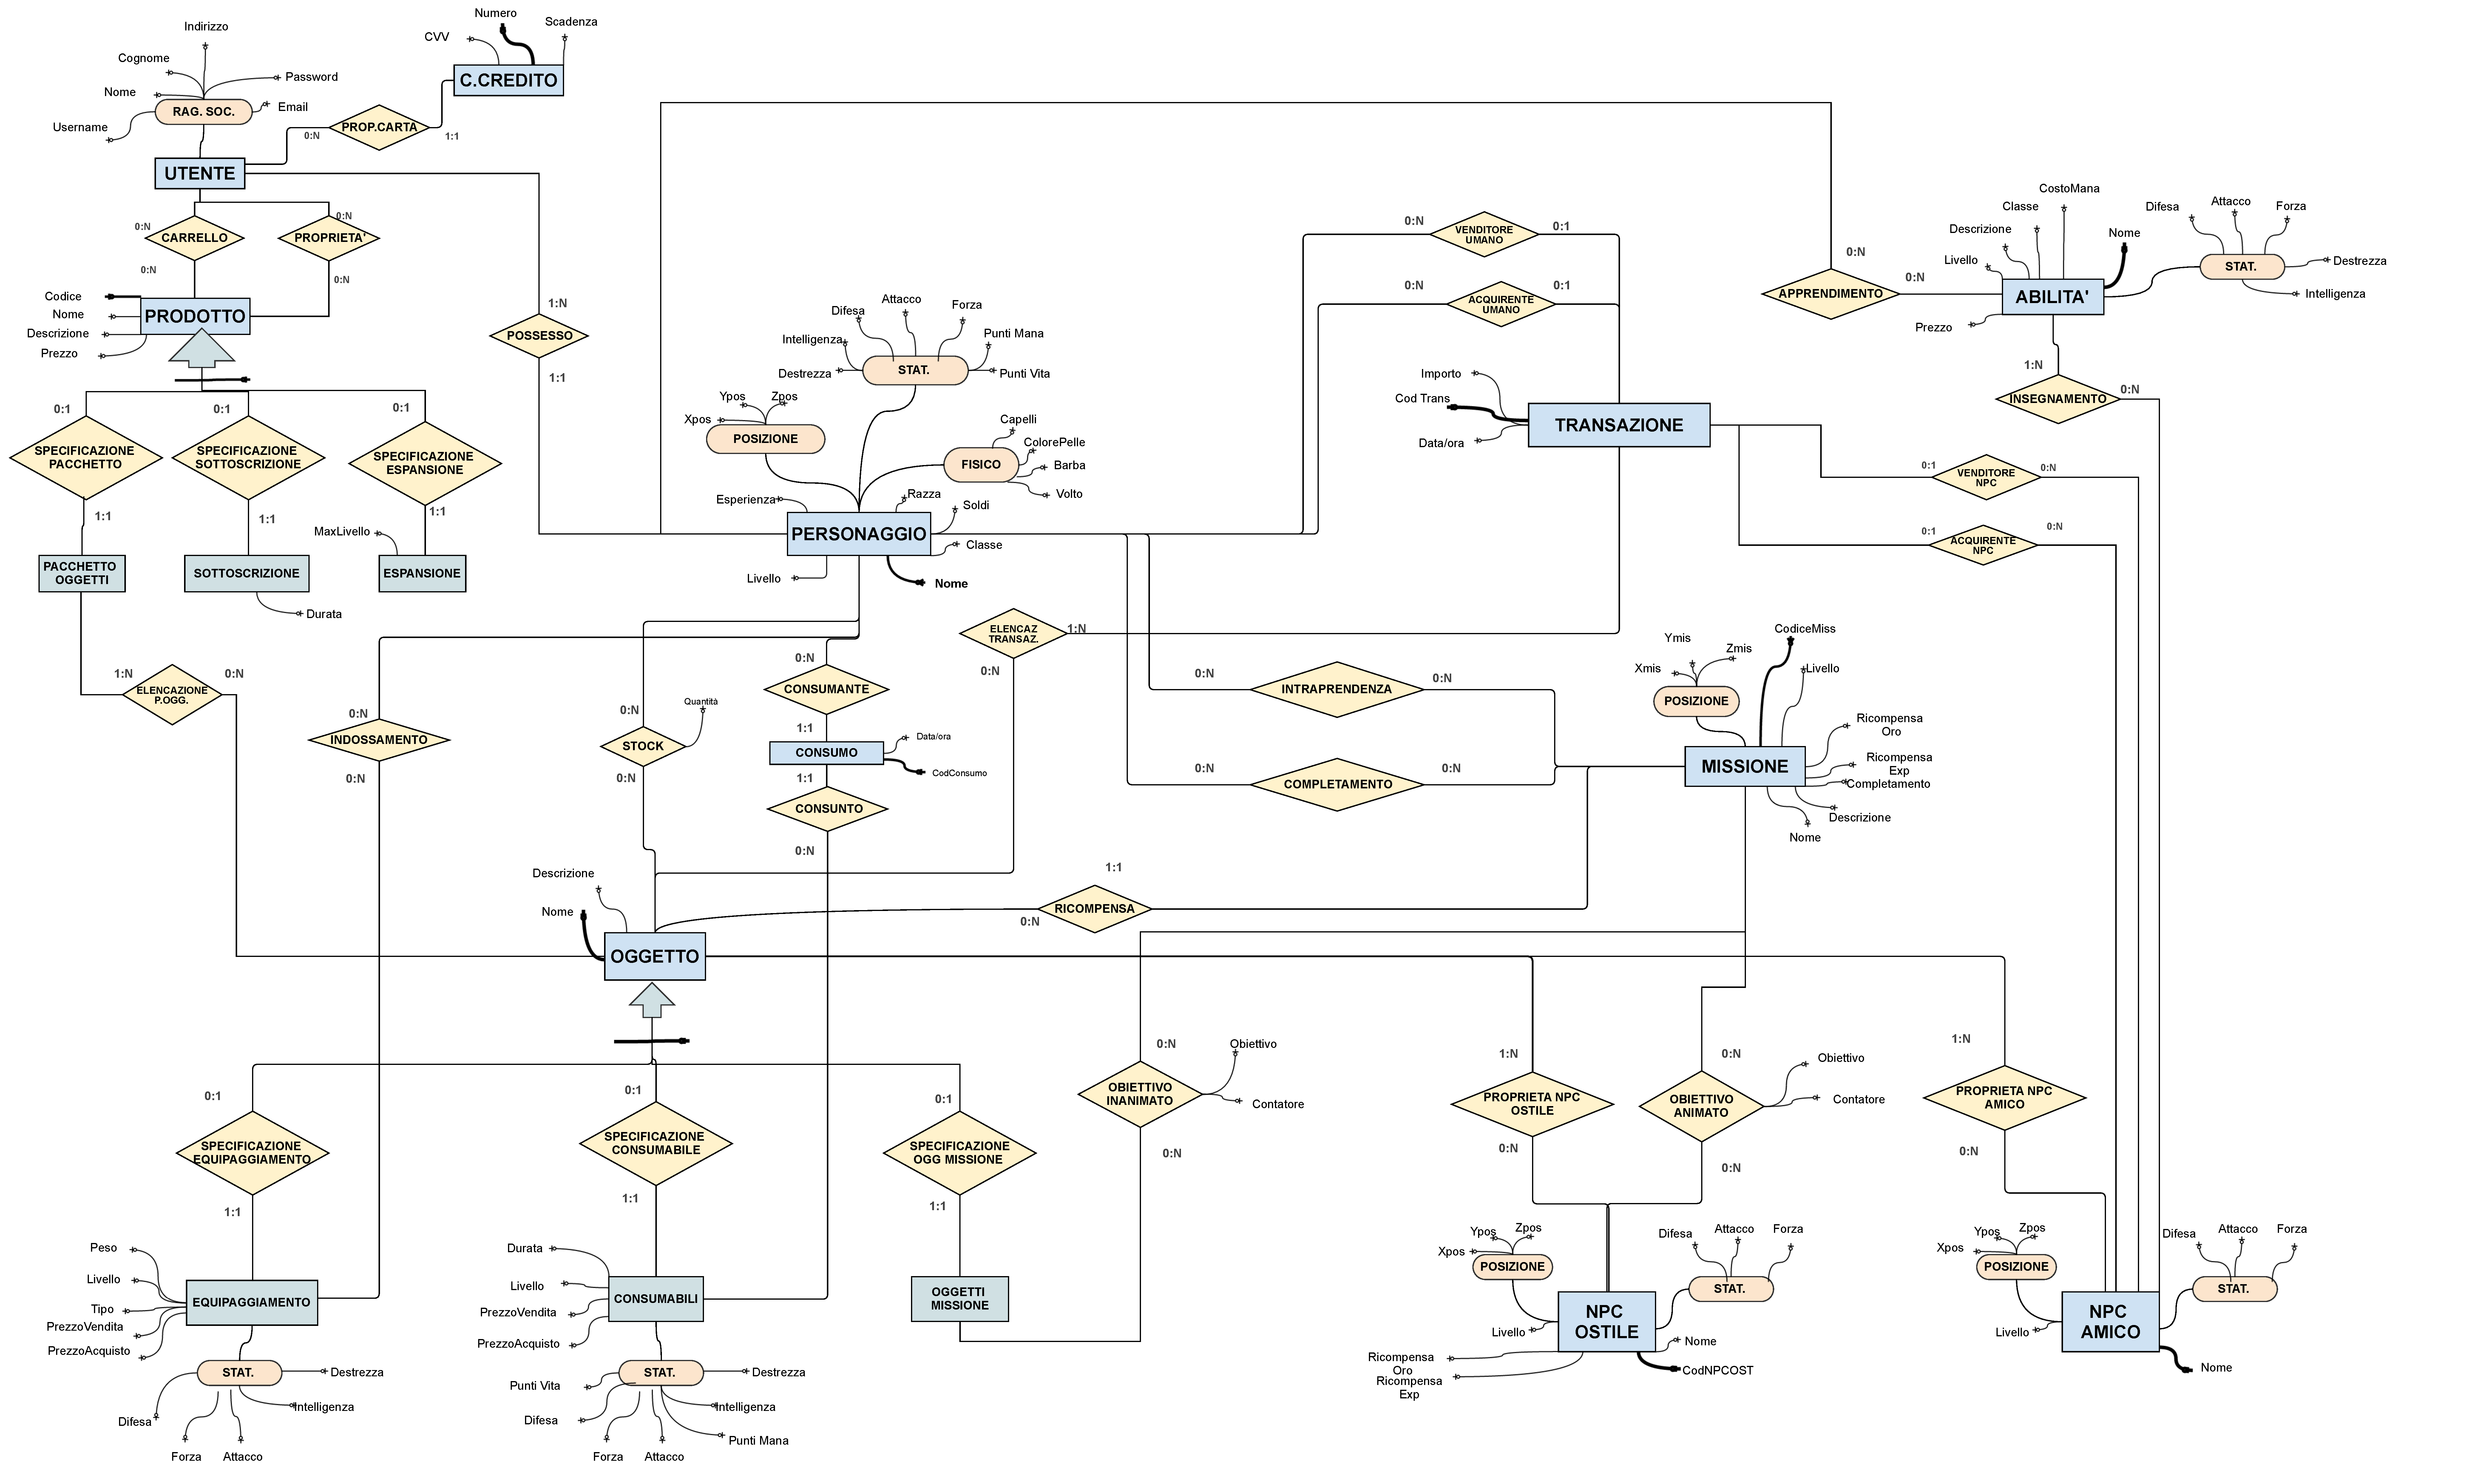
\includepdf[width=270mm, height=210mm, angle=90, keepaspectratio]{./pdf/ristrutturatocarta.pdf}

\end{landscape}